\documentclass[review]{elsarticle}

\usepackage{lineno, hyperref}

\usepackage{graphicx, overpic, mathtools}

\modulolinenumbers[5]

\graphicspath{{Figures/}}
\newcommand{\std}[1]{{\langle {#1}^2\rangle}^{1/2}}
%%%%%%%%%%%%%%%%%%%%%%%%%%%%%%%%%%%%%%%%%%%%%%%%%%%%%%%%%%%%%%%%%%%%%%%%%%%%%%%%%%%%%%%%%%%%%

\usepackage{lineno, hyperref}

\usepackage{graphicx, overpic, mathtools}

%%%%%%%%%%%%%%%%%%%%%%%%%%%%%%%%%%%%%%%%%%%%%%%%%%%%%%%%%%%%%%%%%%%%%%%%%%%%%%%%%%%%%%%%%%%%%

%% Vancouver name/year
\usepackage{numcompress}
\bibliographystyle{model4-names}
\biboptions{authoryear}

%%%%%%%%%%%%%%%%%%%%%%%%%%%%%%%%%%%%%%%%%%%%%%%%%%%%%%%%%%%%%%%%%%%%%%%%%%%%%%%%%%%%%%%%%%%%%

\title{Vortex induced vibrations suppression for a cylinder with plasma actuators}

%%%%%%%%%%%%%%%%%%%%%%%%%%%%%%%%%%%%%%%%%%%%%%%%%%%%%%%%%%%%%%%%%%%%%%%%%%%%%%%%%%%%%%%%%%%%%

\begin{document}

\begin{frontmatter}

\title{Vortex induced vibrations suppression for a cylinder with plasma actuators
%\tnoteref{mytitlenote}
}
%\tnotetext[mytitlenote]{Fully documented templates are available in the elsarticle package on \href{http://www.ctan.org/tex-archive/macros/latex/contrib/elsarticle}{CTAN}.}

%% Group authors per affiliation:

\author[FIUBA]{F. Castro Hebrero \corref{mycorrespondingauthor}}
\cortext[mycorrespondingauthor]{Corresponding author}
\ead{fcastroh@fi.uba.ar, fcastroh@yahoo.com.ar}

%\author[FIUBA]{F. Castro Hebrero \corref{mycorrespondingauthor}} 
\author[FIUBA,CONICET]{J. D'Adamo}
\author[FIUBA,CONICET]{R. Sosa}
\author[FIUBA,CONICET]{G. Artana}

\address[FIUBA]{Fluid Dynamics Laboratory, Buenos Aires University, Argentina.}
\address[CONICET]{National Research Scientific and Technical Council, Argentina.}

%\address[mysecondaryaddress]{Av. Paseo Colón 850, C1063ACV, Ciudad Autónoma de Buenos Aires, Argentina}

%\author{Elsevier\fnref{myfootnote}}
%\address{Radarweg 29, Amsterdam}
%\fntext[myfootnote]{Since 1880.}

%% or include affiliations in footnotes:
%\author[mymainaddress,mysecondaryaddress]{Elsevier Inc}

%\address[mymainaddress]{1600 John F Kennedy Boulevard, Philadelphia}
%\address[mysecondaryaddress]{360 Park Avenue South, New York}

%%%%%%%%%%%%%%%%%%%%%%%

\begin{abstract}
In this research, we propose the use of plasma actuators to control the vortex induced vibration phenomena (VIV) originated by an airflow around a rigid circular cylinder. The body was placed in a closed loop wind tunnel and mounted with elastic supports that allowed small oscillatory movements in the transverse direction with respect to the free stream. Our goal was to suppress the vibrations that occurred naturally in this configuration. To this end, two plasma actuators  were disposed symmetrically on the surface of the cylinder along the span that transferred momentum to the fluid by means of a dielectric barrier discharge. Experiments were performed varying the free stream velocity and the actuation was kept constant all along our experiments as the electrical parameters of control of the actuators, voltage and frequency,  have always been the same. We characterised the dynamics of the system for experimental conditions by involving a high mass ratio $m^* \approx O(10^3)$ and considering  Reynolds numbers   in the intermediate sub critical flow regime $\text{Re} \approx 1 \cdot 10^{3}-10^{4}$. The reduced velocities  lied in the range $4.50 < U_{r} < 6.25$. Our results show that the plasma actuators exhibit a large authority to suppress the VIV in all the range of the experimental conditions tested. Complementary measurements undertaken with a PIV system enabled us to explain the outstanding performance observed.
\end{abstract}

%%%%%%%%%%%%%%%%%%%%%%%

\begin{keyword}
circular cylinder, VIV, plasma actuators, plasma control, forced wakes
\end{keyword}

\end{frontmatter}

%%%%%%%%%%%%%%%%%%%%%%%
\linenumbers
%%%%%%%%%%%%%%%%%
\section{Introduction}
\label{sec:Int}
%%%%%%%%%%%%%%%%%

The flow-induced vibrations of rigid bluff bodies have been largely investigated along the last decades; Nevertheless, most attention was given to the VIV of circular cylinders. This is, in part, due to the engineering importance of circular cross-section bodies and also because the dynamics of the wake of cylinders are considered as a reference flow to describe wakes of more complex bluff bodies.

When Reynolds numbers, $\text{Re}=UD/\nu$, exceeds a threshold value, close to $48$, instabilities develop leading to a time periodic flow configuration known as the BvK\footnote{B\'{e}rnard-von K\'{a}rm\'{a}n} vortex street. For Reynolds number values in proximity of this threshold, the wake is laminar and bi dimensional and gradually becomes 3D as Reynolds number increases. Even though higher harmonics may develop when three-dimensional effects appear ($\text{Re}>180$), the footprint of the fundamental 2D harmonic in the whole dynamics appears indicating its predominance in most of the cases \citep{Dusek1994}. VIV in rigid bodies occurs due to the fact that the shedding of vortices produce an oscillatory excitation to the structure. Depending on the characteristics of the supports, the system may oscillate due to lift or drag, or both types of forces. If the support restricts the movement to the transverse direction with respect to the free stream, the system oscillates only on account of lift forces. In general, the amplitude of transverse VIV, which can exceed a diameter in some cases, is greater than that of in-line VIV \citep{Jauvtis2004}. 

Bodies excited by vortices can experience a nonlinear phenomenon known as lock-in, when vortex shedding becomes synchronised with the natural frequencies of oscillation of the mechanical structure. This synchronisation can lead to an increase in the span wise correlation of the vortex shedding and thus to a substantial amplification of the cylinders vibrational response. When the vortex shedding frequency can be controlled, this lock in phenomena between structure and shedding may be suppressed.

Over the years, controlling or suppressing VIV has drawn considerable attention to economic and technical interests such as enhancing safety, efficient operation or life time of the structures affected by the VIV phenomena. In consequence, various VIV control devices are available. They can be classified into two major categories: passive, where no power input is required; and active, in which power input is demanded \citep{Benard2010}.

Passive VIV control is usually proposed by introducing geometrical changes of the bluff body with helical strake, shroud and tripping wires \citep{Hover2001, Bearman2004, Trim2005, Brankovic2006, Korkischko2010}. The main advantage of passive control methods is that they do not require energy input and,in consequence,they are easy to implement. It is difficult, however, to dramatically reduce the vortex-induced vibration with passive control. Furthermore,  using these devices  often produce  an increase of the mean drag, as shown in \cite{Korkischko2010} and \cite{Zdravkovich1981}. 

Active VIV control methods inject a small and tunable amount of energy to the flow and seems to be a more attractive strategy, as forcing can be adjusted to external modification of system's conditions. On one hand, vortex strength reduction strategies were applied in  wakes in order to attenuate the resulting VIVs. Some examples are: moving surfaces \citep{Korkischko2012}, flush-mounted piezoelectric actuators \citep{Zhang2004}, synthetic jets \citep{Wang2016a}, pure suction \citep{Chen2014} or blowing devices \citep{Skaugset2003}, windward-suction-leeward-blowing (WSLB) \citep{Wang2016b}, rotational oscillations \citep{Du2015}, travelling wave wall devices \citep{Xu2014}, and actuators based on  Lorentz forces (MHD) \citep{Chen2005}.

On the other hand, VIV can also be mitigated by shifting the vortex shedding frequency away from the natural frequency of the body structures \citep{Wang2017, Du2015}. One possibility here is to consider devices that impose a periodic forcing to the flow. However, this strategy based on a synchronisation between forcing and shedding may be quite difficult. The flow dynamics in general may be driven by periodic external forces of reduced amplitude only within a narrow band of frequencies around the natural vortex shedding frequency. To introduce significant changes in the vortex shedding frequency, it may be more effective to propose another strategy based on another concept. Rather than driving the flow to a forcing frequency, it may be more effective to produce modifications of the base flow. It has previously been established that the base flow for cylinder wake studies is the averaged time flow \citep{Barkley2006}, so its changes  determine the characteristics of the instabilities that develop.  Therefore, in such case one possible strategy for VIV control is to force the flow in order to modify the mean flow. In this research, we rely on this last strategy to suppress the VIV.

It is clear that forcing technology is a central aspect for VIV. Although plasma actuators have rapidly developed over the last 30 years in the flow control community (for instance, the pioneer works of \cite{Roth2000, Artana1999} denotes this or the comprehensive reviews in \cite{Moreau2007, Corke2010, Wang2013}) according to our knowledge, only the work of \cite{Sari2010} has tried to control VIV by plasma actuation. On the contrary, in the aeroacoustic field, different authors proposed these devices to control the aerodynamic noise in geometries like cylinders (Thomas, AIAA JOURNAL Vol. 46, No. 8, August 2008; Huang, Zang Li, J Sound Vibration 2010, Kopien et al J Physics D: Apllied Physics 2017 ) cavity flows (Huang Zang POF 2008)  or flat plates (Al Sadawi, Chong, Kim J Sound Vibration 2019)

Plasma actuators show unique properties in terms of flow manipulation as: momentum addition close to the wall, no moving parts, short command to action delays (of the order of the $1\mu seg$) and high geometric versatility, allowing mounting on any surface exposed to the flow. Most of these actuators use non-thermal surface plasmas in which the air flowing close to the wall of a body is weakly ionised. Due to the presence of charged particles within a highly non-uniform electric field and through a collisional mechanism, the plasma can create a body force close to the electrode surface. Consequently, this is a forcing without addition of mass. The coupling flow discharge is not only restricted to a collisional mechanism, as heating by Joule effects of the fluid particles flowing in proximity of the actuators produce slight modifications of physical properties, as density or viscosity, of these particles \citep{Jayaraman2007}.

The different discharge configurations determine the stability of the discharge, the electrode degradation, the electric force distribution or the energy consumption required to attain a given forcing. The most popular of these devices is the dielectric barrier discharge (DBD) actuator, which has been used to achieve control of diverse flows, exhibiting the following as strong advantages: a simple implementation, reproducible performances and relative robustness. Given that the forcing results quite localized (a few millimetres from the border of the exposed electrode) this kind of discharge has largely been applied to different laboratory tests of flow control studies. With the DBD actuators the discharge is produced by applying a high voltage AC signal to a pair of electrodes that are separated by a dielectric layer. Typically, the voltage magnitude is a few $kV$, the AC frequency is a few $kHz$, and the dielectric layer is of thickness $0.1-1 mm$. Under these conditions stable surface plasma, consuming tens of watts per meter of electrode, can be easily created at atmospheric pressure. The amplitude control parameter can be directly adjusted in a relative small range by means of the high voltage AC signal amplitude. These actuators not only force the flow, but also the structure simultaneously. The ionic wind they induce, produce a reaction (thrust) that forces the structure in opposite direction to the induced flow. The  phenomena is similar to the one well described in \cite{Loeb1939} for the ionic wind with a corona discharge wheel device. This force has been measured by different authors and its value is of the order of a few tens of $mN/m$. 

The objective of the present work is to analyze the authority of these DBD plasma actuators to suppress the VIV of a cylinder wake flow and to try to explain how this is produced.

%%%%%%%%%%%%%%%%%
\section{Experimental setup}
\label{sec:Exp}
%%%%%%%%%%%%%%%%%

In the present investigation, we consider a smooth hollow rigid cylinder of PMMA with an external diameter of $D=0.030 m$, a length of $L = 0.450 m$ and a wall thickness of $3mm$. The mass of this cylinder was $0.204 kg$.

The cylinder was mounted inside the low turbulence \textit{Tango Wind Tunnel} of the \textit{LFD}\footnote{\textit{Fluid Dynamics Laboratory}} \citep{dadamo2017}. The wind tunnel square test section has a side width $B = 0.455 m$ and a total streamwise length of $0.910 m$. The gap between the cylinder ends and the tunnel walls were $2.5 mm$. No correction associated to blockage effect was done.

\begin{figure}[h]
\centering
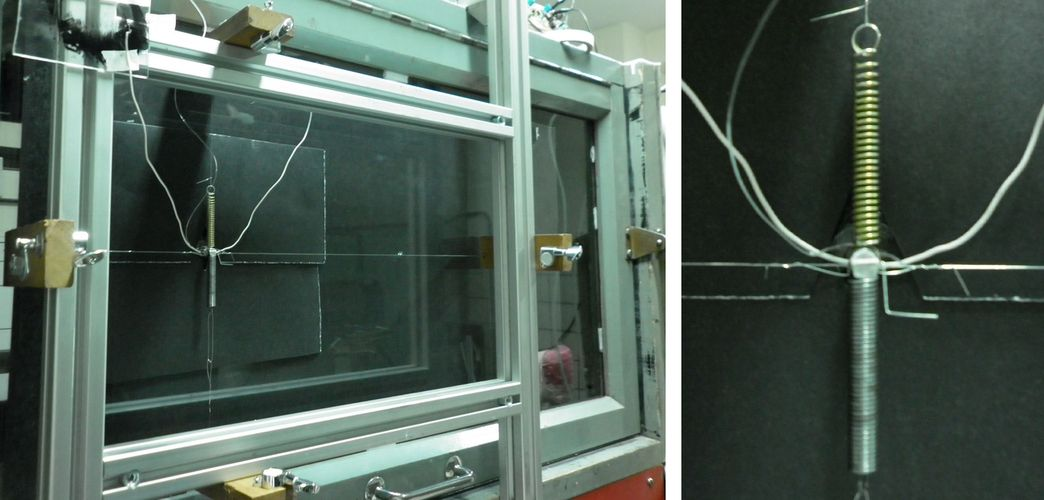
\includegraphics[width=0.75\textwidth]{Figures/Fig_01}
\caption{Left: Wind Tunnel with an external structure. Right: detail of the vertical pair of linear springs, horizontal guitar string to calibrate and plasma electric wiring mounted outside the test section.}
\label{fig:01}
\end{figure}

The flow velocity was varied between  $U= 3.00 - 4.25 m/s$ ($6000<\text{Re}<8500$) during the experiments. According to the classification of \cite{Williamson1996}, this cylinder wake flow belongs to the so called Shear-Layer Transition Regime. This incoming free stream flow had fluctuations around the mean value lower than $\pm 2\%$. The associated reduced velocity, $U_r = U / f_s^0 D$, where $f_s^0$ is the structure natural frequency, was thus varied between $4.50$ and $6.25$. 

As for the range of Reynolds numbers considered, the expected Strouhal number is $\text{St}=f_{vs}D/U \approx 0.208$ \citep{Fey98}, with $f_{vs}$ as the vortex shedding frequency. The flow we analyzed has also been associated to a periodic detachment of transition eddies along the free shear layer. The frequency of formation  of these eddies depend on Reynolds number. Typical frequencies of the transition eddies are close to 5 or 6 times the one of vortex shedding and, in our case, this corresponds to values that are larger than $150 Hz$.

The cylinder was elastically mounted using four (two for each side) linear springs disposed outside the test section. Stressed chord wiring were also used in order to restrain the cylinder movement, enabling only significant movements in the transverse direction with respect to the flow. This particular arrangement is suitably fitted in order to produce low structural damping (Fig. \ref{fig:01}). The tunnel window possesses small grooves to allow the movement of the cylinder; fluid leaks are negligible.

\subsection*{Cylinder and flow dynamics}

The transverse displacement of the cylinder was measured with an inductive displacement sensor with digital output (TURCK  NI8-M18-LIU). The sensitivity of the sensor in distance is $0.04mm$. Its signal was captured by an oscilloscope (RIGOL $50 MHz$, 4 channels) and the processing of the signal enabled us to obtain the frequency and the spectrum of energy of the cylinder oscillations.

A 2D PIV acquisition system was used to obtain the  flow field at the mid-span of the cylinder.  Image acquisition and PIV calculations were performed using a LaVision system, composed of an ImagerPro $1200 \times 1600$ CCD camera with a 14-bit dynamic range capable of recording double-frame pairs of images at 8 Hz and a two-rod Nd:YAG (15 mJ) pulsed laser synchronized by a customized PC using LaVision DaVis 7.1 software. The field of view of the experiment was of $175.5mm  \times  234.0mm$ (about $5.85 D \times  7.8 D$). During post-processing of the images with the PIV algorithm, this region was divided into interrogation cells of $16  \times  16$ pixels$^2$ with an overlapping of $50 \% $ giving a spatial resolution of the vector fields of $0.078D$. The maximum sampling frequency of the system is about $14,8 Hz$ and with the assumed $\text{St}\simeq 0.208$, we obtain $f_{vs} > 20Hz$, and thus the flow field dynamics was sub-sampled on time.

\subsection*{Plasma actuation characteristics}

The plasma actuators geometry is shown in  Figure \ref{fig:02}. The span of the actuator is $80\%$ of the length of the cylinder. The electrodes were made with aluminum tape and the dielectric was made with $3$ layers of Kapton tape of thickness $3 x 60\mu m = 180\mu m$ (Polyimide Film Tape with $6kV$ of dielectric strength). The width of the insulated electrode (internal) is $6$mm and of the exposed electrode (external) is $10$mm. The actuators were disposed blowing in the downstream direction as it is schematically showed in Fig. \ref{fig:02}. The downstream edges of the exposed electrodes are placed at $\pm 90^\circ$ measured from the upstream stagnation point. With this setup, the electric thrust is negligible as forcing mechanism of the structure in the transverse direction. 

\begin{figure}[h]
\begin{minipage}[c]{\textwidth}
\begin{minipage}[l]{0.475 \textwidth}
\begin{center}
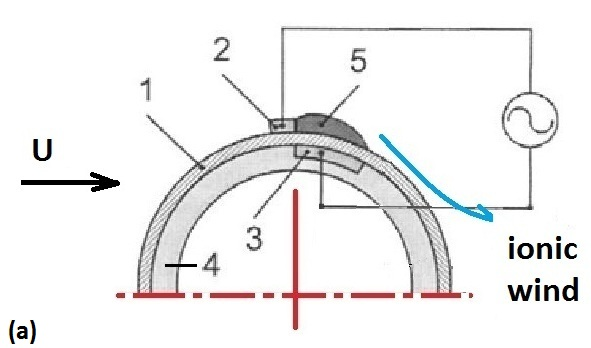
\includegraphics[width = 0.9\textwidth]{Figures/Fig_02_a.jpg}
\end{center}
\end{minipage} \hspace{0.05 \textwidth}
\begin{minipage}[r]{0.475 \textwidth}
\begin{center}
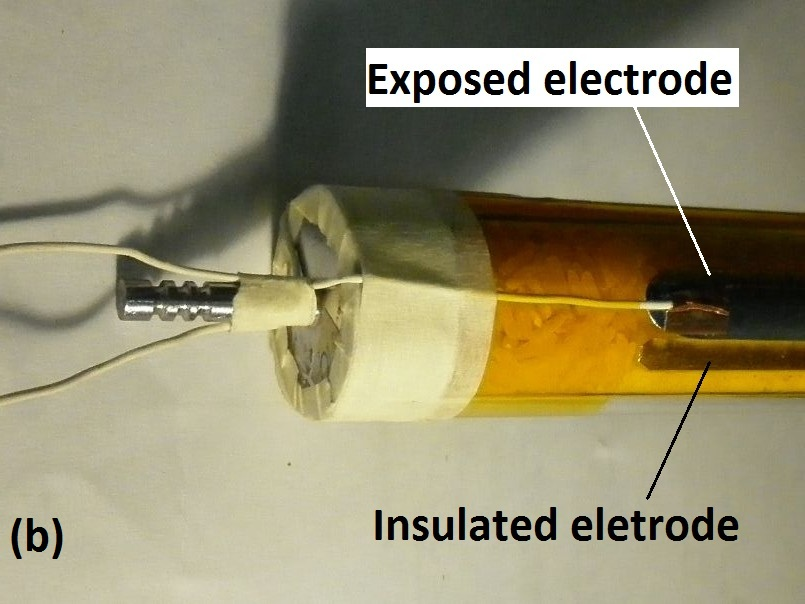
\includegraphics[width = 0.8 \textwidth]{Figures/Fig_02_b}
\end{center}
\end{minipage}
\caption{(a) 1- Kapton, 2- Exposed electrode, 3- Insulated electrode, 4- Cylinder and 5- Plasma. (b) End of the cylinder and electrical terminals of the plasma actuator.}
\label{fig:02}
\end{minipage}
\end{figure}

The electric circuit that excites the electrode is composed of a signal generator, an audio amplifier and an ignition coil. The voltage was set to $V_{ehd} \approx 12 \text{kV}_{pp}$ and frequency of the AC signal was $f_{plasma} \approx 2 kHz$. In our experiments these parameters of operation have always been the same. The power consumption of the actuators is approximately $20-25 W/m$, so for the aforementioned span, it is about $14.4-18.0 W$. Usually, only a fraction lower than $10\%$ of this power is transformed into mechanical power supplied to the flow by the actuator \citep{Moreau2007}.

\subsection*{Non dimensional parameters}

Our mechanical system can be analyzed as an  elastically supported rigid circular cylinder of diameter $D$ and length $L$ with one degree of freedom. When it faces a stationary and uniform flow of free stream velocity $U$,  the cylinder can oscillate transversely as illustrated in Fig. \ref{fig:03}.

\begin{figure}[h]
\centering
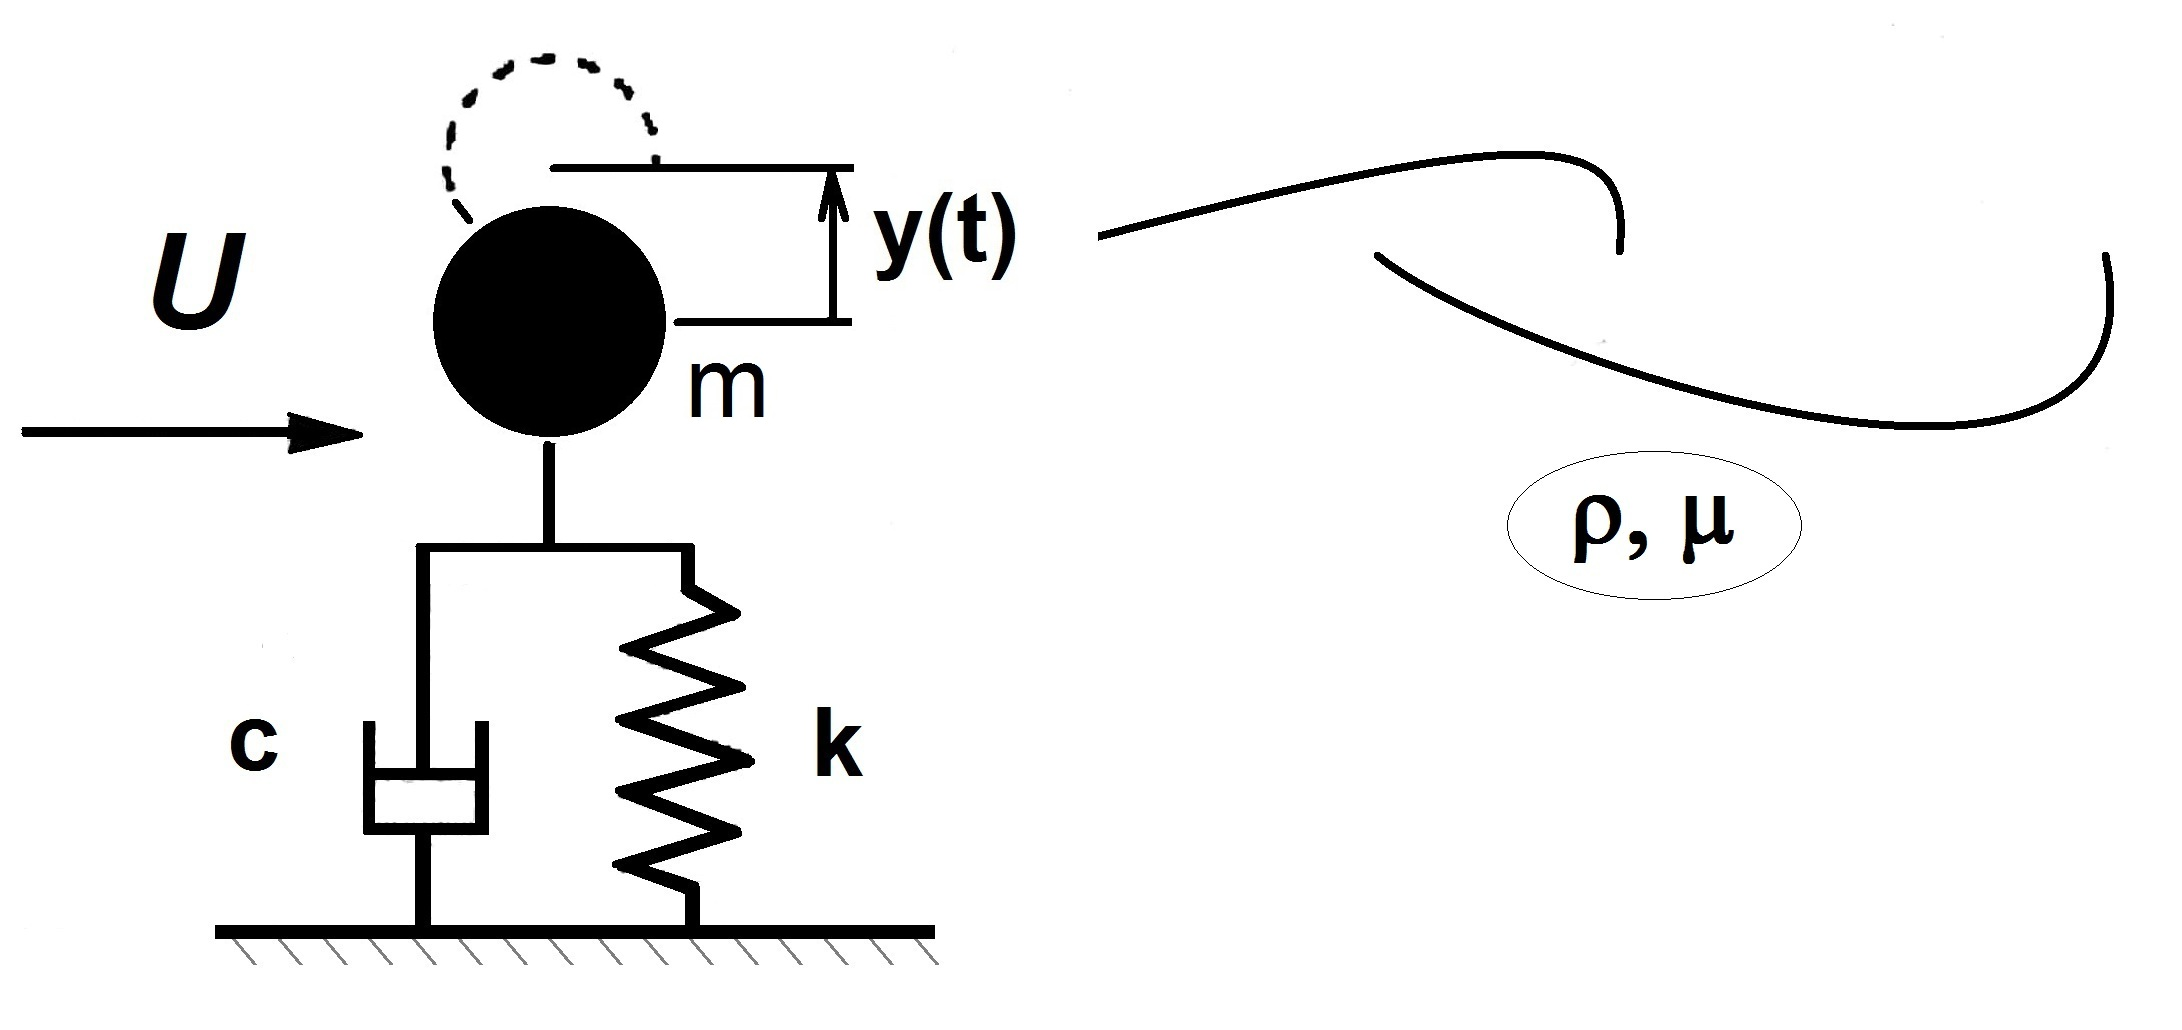
\includegraphics[width = 0.6 \textwidth]{Figures/Fig_03}
\caption{System configuration for an elastically-mounted, rigid cylinder in a uniform flow.} %\cite{LANGREBOOK}
\label{fig:03}
\end{figure}

The dimensional in-plane cross-flow displacement $y(t)$ of the structure is described by the following expression that portrays the dynamics of a linear oscillator

\begin{equation}
m \frac{d^2y}{dt^2} + c \frac{dy}{dt} + k y = F~,
\label{eq:model}
\end{equation}

Where $m$ is the total oscillating structural mass, $c$ the structural damping, $k$ the structural stiffness, $F \equiv F_{(t)}$ the force in the transverse direction. The structural stiffness $k$ of our setup was measured with a static calibration using reference masses. It was found to be $885 ~\pm ~20$ $N/m$ by spring. On the other hand, the natural frequency ($f_{s}^{0}$) and the structural damping coefficient ($\xi$) were determined experimentally by means of a series of decay test in still air.

The model schematised in Figure \ref{fig:03} is compatible with an identical and vertical in phase movement of both elastic supports of the cylinder. As opposite phase movement is not restricted with our set up we have determined the natural frequency oscillation in which both ends of the cylinder are not in phase (tilted mode). The frequency of the tilted mode was close to $35.5 Hz$. The measured frequencies of oscillation in our experiments were rather far from this value and  so the model proposed seems to be adequate to describe the dynamics of our system.

Thus, the motion of the cylinder, $y(t)$, that results from the coupling with the wake can be analyzed in terms of the simple variables: the amplitude $A$ and  frequency $f_s$ of vibration. The dynamics of the flow bring as additional variable to the analysis, the dominant frequency of vortex shedding, $f_{vs}$. These variables, $A$, $f_ s$ ,$ f_{vs}$, describe separately the characteristics of the dynamics of the fluid and of the structure, but are actually coupled. 

This reads, in a general form

\begin{equation}
[A, ~ f_s, ~ f_{vs}] = \mathcal{F} \left(m, ~ c, ~ k, ~ U, ~ \rho, ~ \mu, ~ D \right)
\end{equation}

At this stage, because of the large number of parameters involved, some dimensional analysis is necessary. In dimensionless form,

\begin{equation}
\left[ \frac{A}{D}, ~ \frac{f_s}{f_s^o}, ~ \frac{f_{vs}}{f_s^o} \right] =  \mathcal{F}^* \left(\frac{UD\rho}{\mu}, ~ \frac{U}{f_s^o D}, ~ \frac{m}{\rho L \pi D^2 / 4}, ~ \xi \right)
\end{equation}

The dimensionless groups on the right-hand side are the Reynolds number, the reduced velocity, the reduced mass and the structural damping coefficient in still fluid ($\xi=c/4\pi m f_s^o$), where the natural frequency in still fluid, $f_{s}^{0}$, is defined as $\omega_s^o = 2\pi f_s^o = \sqrt{k/m}$.

The framework of our experimental study is given by the values adopted by these non-dimensional parameters. 

Table \ref{tab:01} shows the experimentally obtained structural parameters. As is usual with VIV studies undertaken with air flows, the reduced mass adopts relatively high values which in our case was $m^{*} =  523.5 \approx 5 \cdot 10^2$. One can notice that although the system has a high mass ratio, $m^*$, the low damping ratio $\xi$ leads to a relatively small Scruton number ($S_C =m^*. \xi$)  that is a key parameter in the observation of vortex shedding vibrations \citep{Blevins1990}.

\begin{table}[h]
\centering
\begin{tabular}{|c|c|c|c|}
\hline
Symbol & Description & Dimension & Value \\
\hline	
$k$ & structural stiffness & $N/m$ & $3540 ~\pm ~80$ \\
\hline
$f_{s}^{0}$ & natural frequency & $Hz$ & $ 22.7 ~\pm ~0.5$ \\
\hline	
$\xi$ & damping coefficient & $-$ & $ 8.3 ~ \pm ~ 0.5 ~ (\cdot ~10^{-3})$\\
\hline
\end{tabular}
\caption{Structural parameters}
\label{tab:01}
\end{table}

The vortex shedding frequency appears in eq. (\ref{eq:model}) through the forcing term $F$ incorporating a time depending on the excitation to the structure associated to the flow. There may be other frequencies of excitation of the structure associated to the flow. The transition eddies may also excite the structure but these vortices have a strength much lower to the one of vortex shedding, and they also have an associated frequency much larger than the one of interest in our analysis. Thus, in a first analysis their effect can be disregarded.

Also, as regards the cases in which a control is proposed, plasma actuation forces the flow but this occurs only when discharge takes place. This corresponds to a limited part of the cycle of the electric excitation signal. Moreover, the discharge may be considered as a pulsed forcing that takes place recurrently with frequency $f_{plasma}$ but that it is not continuous. This actually introduces a forcing to the flow with a cyclic behaviour. Measurements of spectra of velocities belonging to different forced flows, in proximity of actuation with this kind of actuators show, in general, peaks in agreement with this frequency of excitation. We stand for the idea that it is of high interest to analyse if this frequency may have a significant role in our study or not. In order to achieve this, it is convenient to define two other non dimensional parameters $f_{plasma}/f_s^o $ and $f_{plasma}/f_{vs}$. In our case, both ratio are quite far from unity ($f_{plasma}/f_s^o \sim f_{plasma}/f_{vs} \sim 100$). Thus, the resonance of the structure is quite far from the frequency of excitation that the actuator produces and instabilities of the flow that may be excited by the forcing also have quite lower values. So, we can conclude that the influence of the ``high'' frequency of the forcing will not significantly be observed in the ``slow'' dynamic behaviour of the system analysed.

In summation, in our study $D$, $L$, $m$, $c$ and $k$ are constants (thus with fixed values of $\xi$ and  $m^*$) and changes in the natural VIV phenomena can be achieved only as a consequence of changes in the uniform fluid stream.The forcing parameters are also kept constant. Hence, the characteristics of the dynamics  will be governed only by two non-dimensional numbers, the Reynolds number ($\text{Re}$) and the reduced velocity ($U_r$). 

%%%%%%%%%%%%%%%%%
\section{Results}
\label{sec:Res}
%%%%%%%%%%%%%%%%%

\subsection*{Transverse Cylinder oscillations}

Figure \ref{fig:04}a) shows a typical signal obtained with the displacement sensor and Fig. \ref{fig:04}c) the associated Fourier energy spectrum. In all the experiments the transverse displacement amplitude of the cylinder was obtained as the root mean square of the displacement signal ($A \equiv A_{rms}$), and the frequency of the cylinder oscillations ($f_s$) was obtained from the Fourier frequency spectrum of the signal. The recorded signal shows a high frequency signal whose amplitude is modulated by a low frequency. Figure \ref{fig:04}b) shows a {\it linear-log} graph zoom of the Fourier energy spectrum. The spectrum shows that in the cylinder oscillation there exists a dominant frequency but there may appear a significant contribution to the signal given by oscillation modes (first peak) with another frequency at proximity to the dominant one (secondary peak). Figure \ref{fig:04}c) enables a global observation of the spectrum. The third peak appearing at proximity of $35.5Hz$ corresponds to the tilted movement mode. Finally, harmonics of the first two peaks appear close to $44.5Hz$.

\begin{figure}[h]
\begin{minipage}[c]{\textwidth}
\begin{center}
\begin{minipage}[r]{0.48\textwidth}
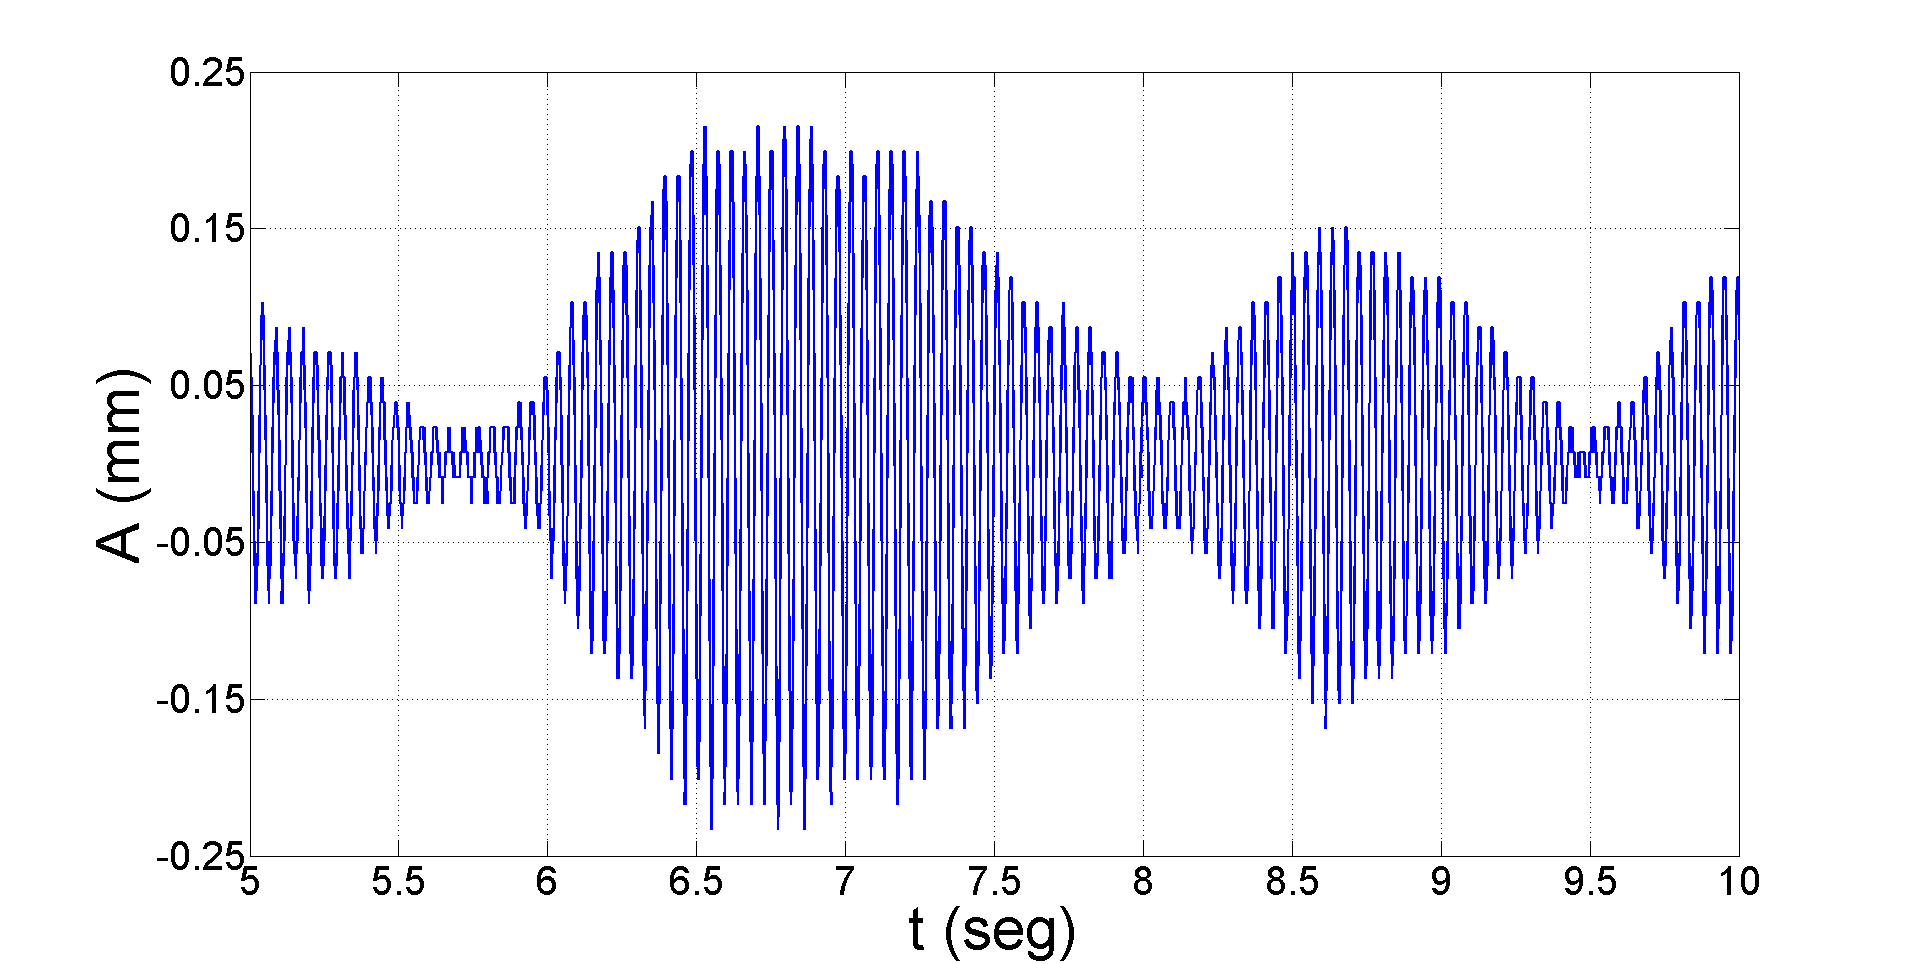
\includegraphics[width=1\textwidth]{Figures/Fig_04_a}\\
{\footnotesize a)}
\end{minipage}\begin{minipage}[l]{0.52\textwidth}
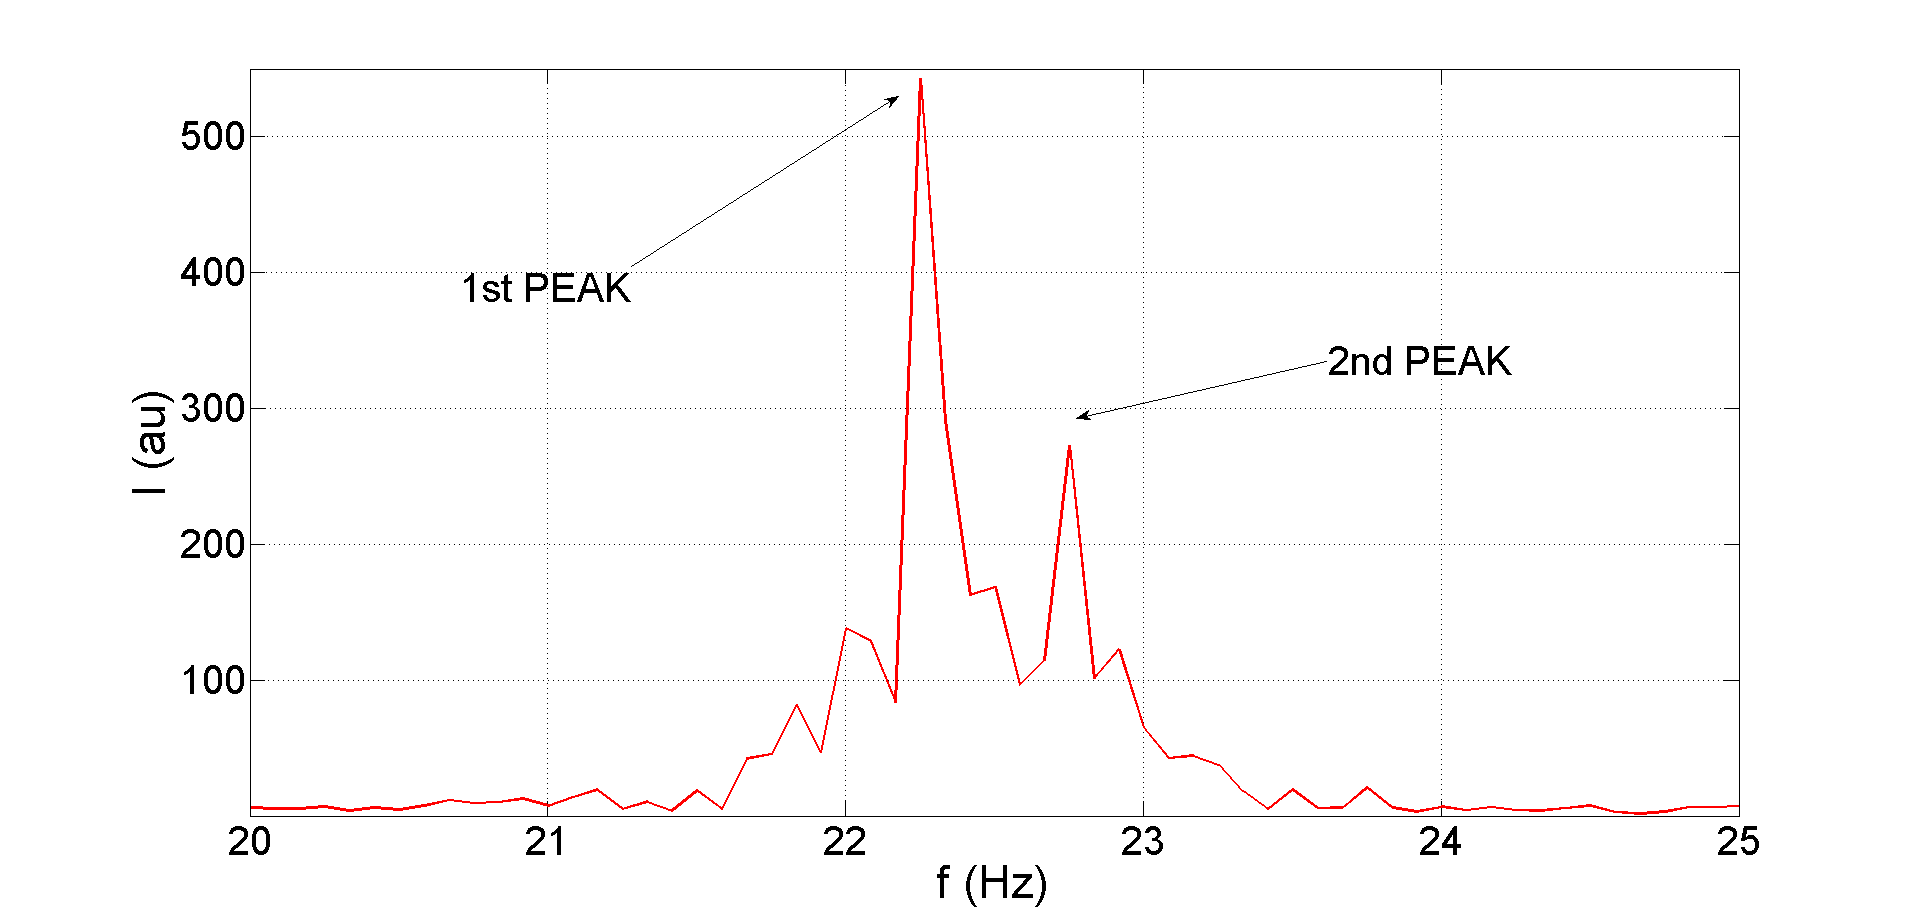
\includegraphics[width=\textwidth]{Figures/Fig_04_b}\\
{\footnotesize b)}
\end{minipage}
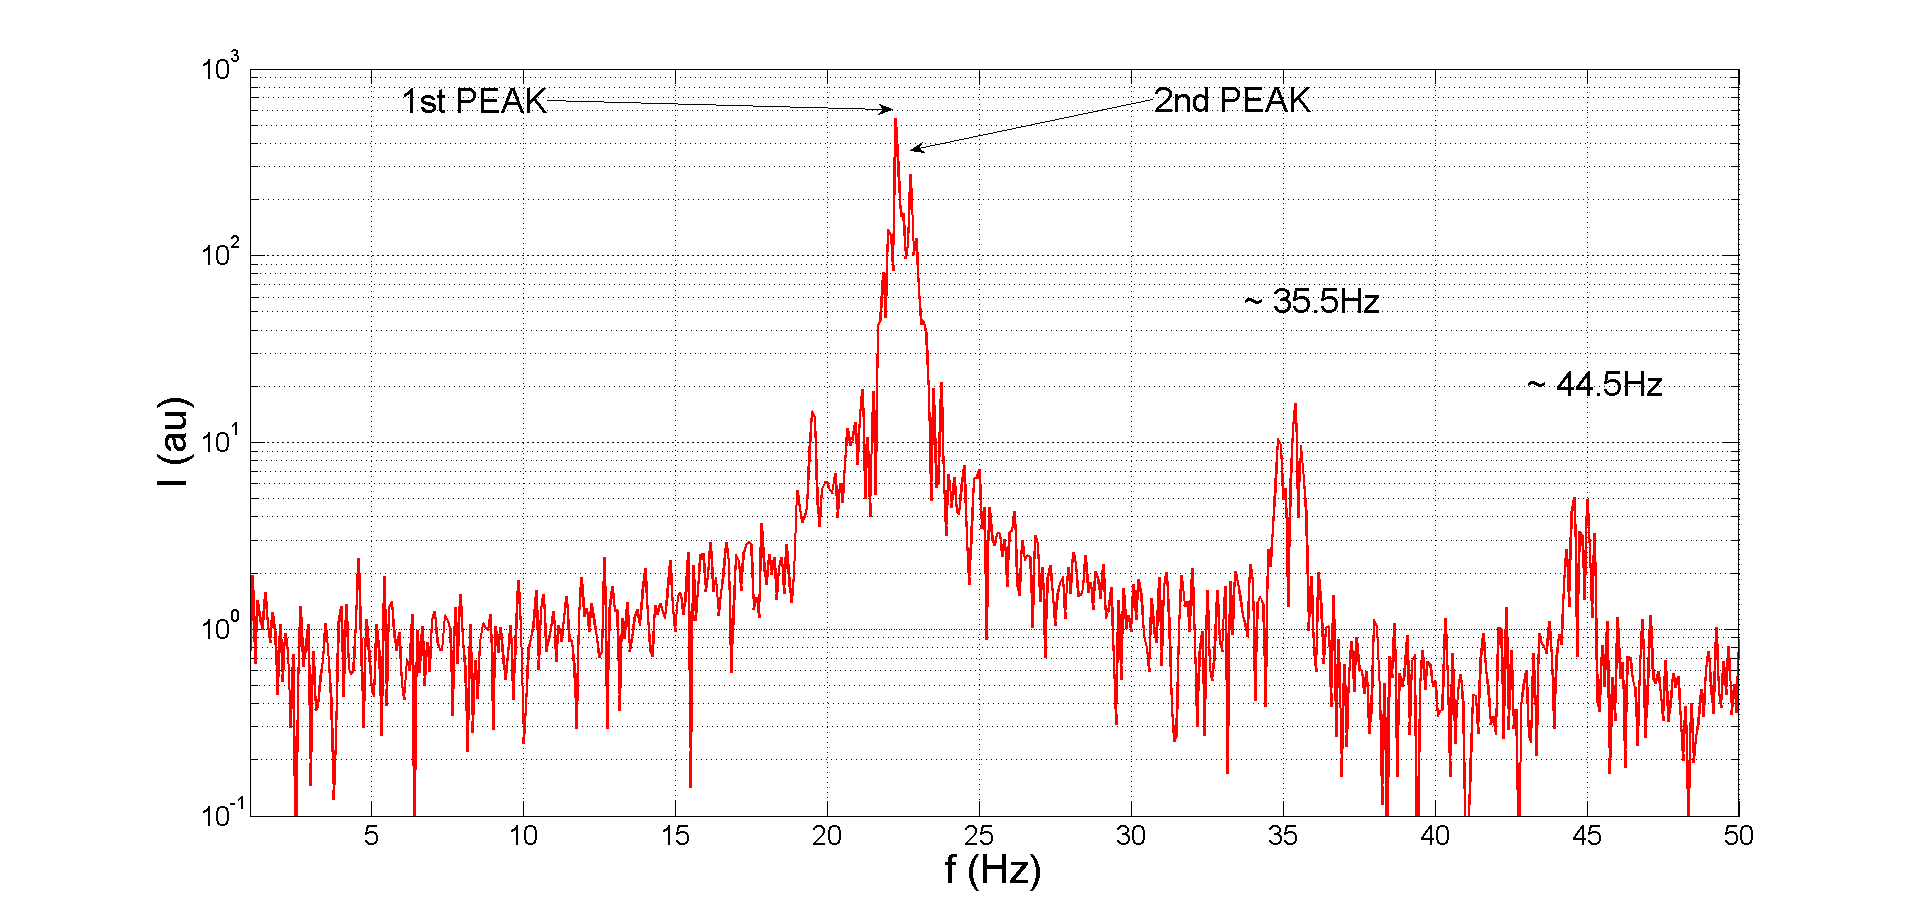
\includegraphics[width=1\textwidth]{Figures/Fig_04_c}
\begin{flushleft}
{\footnotesize c)}
\end{flushleft}
%%%%%%%%%%%%%%%%%%%%%%
\caption{$U \approx 3.85 m/s$. 
a) Signal obtained with the displacement sensor. $Sampling=1000Hz$ and $t_{total} = 7seg$.
b) {\it linear-log} spectrum graph. $1^{st}$ Peak: $f_{1} = 22.25Hz$ and $E_1 = 542a.u.$ $2^{nd}$ Peak: $f_{2} = 22.75Hz$ and $E_2 = 270 a.u.$ 
c) Fundamental frequency of tilted movement $\sim 35.5Hz$ and first harmonic $\sim 44.5Hz$.}
\label{fig:04}
\end{center}
\end{minipage}
\end{figure}

Figure \ref{fig:05} shows the dimensionless amplitude ($A^* =A / D$) and frequency ($f^* = f_s / f_s^o$) of the cylinder oscillations in terms of the reduced velocity for the controlled ({\it Plasma-on}) and non-controlled ({\it Plasma-off})  cases respectively. Within our experimental conditions, the cylinder displacements without any forcing  has shown a relative dispersion of results among experiments.

In order to find  representative results we have performed more than thirty experiments for the unforced case. In Fig. \ref{fig:05}  we show four curves for the uncontrolled VIV phenomena. All the experimental data of $A^*(U_r)$ was found to lie between the {\it Plasma-off max} curve and the {\it Plasma-off min} curve. In the same graph we have also plotted the averaged value  {\it Plasma-off mean}. A reference result corresponding to a single experiment in which we varied continuously the free airstream velocity is indicated as {\it Plasma-off} with black circles. This figure shows that no vibrations occur for $U_r < 4.75$. On increasing $U_r$, the amplitude rises sharply to a maximum amplitude value.

The maximum response is confined to quite a narrow reduced velocity range, $4.75 < U_r < 5.5$, which is typical of moderate to high-mass-ratio VIV and the maximum is centred upon $U_r \approx 5.15 \approx 1/\text{St}$ \citep{Blevins1990}. By further increasing the velocity of the free airstream, and in consequence of the reduced velocity, we observed that a second local maximum may occur in proximity of the value of $U_r=6$.

Figure \ref{fig:06} shows the non-dimensional frequency response ($f^*= f_s / f_s^o$) of the {\it Plasma off} cases in which  the frequencies $f_s $ were obtained by identifying the most energetic peaks in the energy spectra of the cylinders displacement signal and then dividing by $f_s^o$ (resulting the circles in fig. \ref{fig:06}). It can be seen that the measured main frequency of the cylinder oscillation corresponds to the natural frequency of the structure in still fluid ($f^* \approx 1$ thus $f_s \approx f_s^o$). For each spectrum, we have also selected a second mode of oscillation having an associated peak in the spectrum with a value exceeding $10\%$ of that of the most energetic. In Fig. \ref{fig:06} they are signalled with square symbols for the case taken as reference. These second peaks occur only for $U_r$ values quite away from the natural frequencies of the structure. A linear fitting of the different values of these peaks obtained for all experiments can be proposed. The slope of this curve enables to calculate a Strouhal number.

The fitting gives a $\text{St} \approx 0.198$ (see Fig. \ref{fig:06} b)) quite close to Strouhal number $\text{St} \approx 0.208$ quoted in the literature for a fixed cylinder under this flow conditions.

Considering now the {\it Plasma-on} case, the plasma actuation flattens the spectrum energy and  cancels the oscillations for all the different velocities tested as can be observed in Fig. \ref{fig:05}. It is important to mention that contrary to what was observed for the {\it Plasma-off} case, when the flow is actuated, the curves $A^*(U_r)$ show a very repetitive behaviour. Thus, for these conditions, the amount of data required to characterise the flow control effect was considerably lower than for the non-actuated case. In order to have a better insight on the physics that can explain this outstanding result, we performed PIV experiments to have access to the dynamics of the fluid.

\begin{figure}[h]
\centering
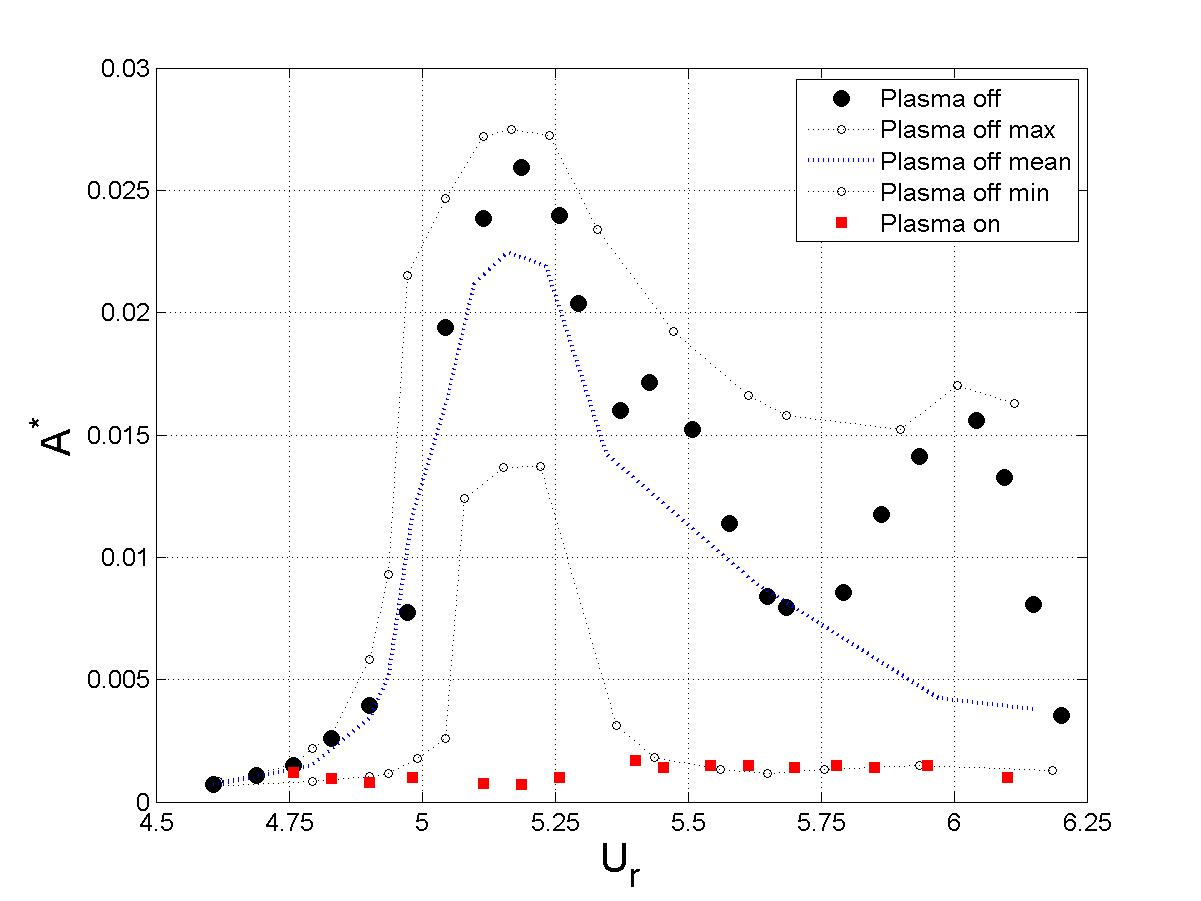
\includegraphics[width=0.9\textwidth]{Figures/Fig_05}
\caption{$A^*$ v.s $U_{r}$.}
\label{fig:05}
\end{figure}

In \cite{Willden2006} the dependency of circular cylinders VIV on their mass ratio (within  the range $1<m^*<50$) and for a relative low Reynolds numbers range $ 50 <\text{Re} < 400 $ was studied. For the cases with the higher values of mass ratio, it has been found a primary response region normally associated with VIV and also a secondary  region was observed in the same sense as we did. Even though the ranges of Reynolds numbers and mass ratio are not the same in both cases, the results illustrated in Figure \ref{fig:05} show a similar behaviour as the one observed in \cite{Willden2006}.

\begin{figure}[h]
\begin{center}
\begin{minipage}[c]{\textwidth}
\begin{minipage}[l]{0.5\textwidth}
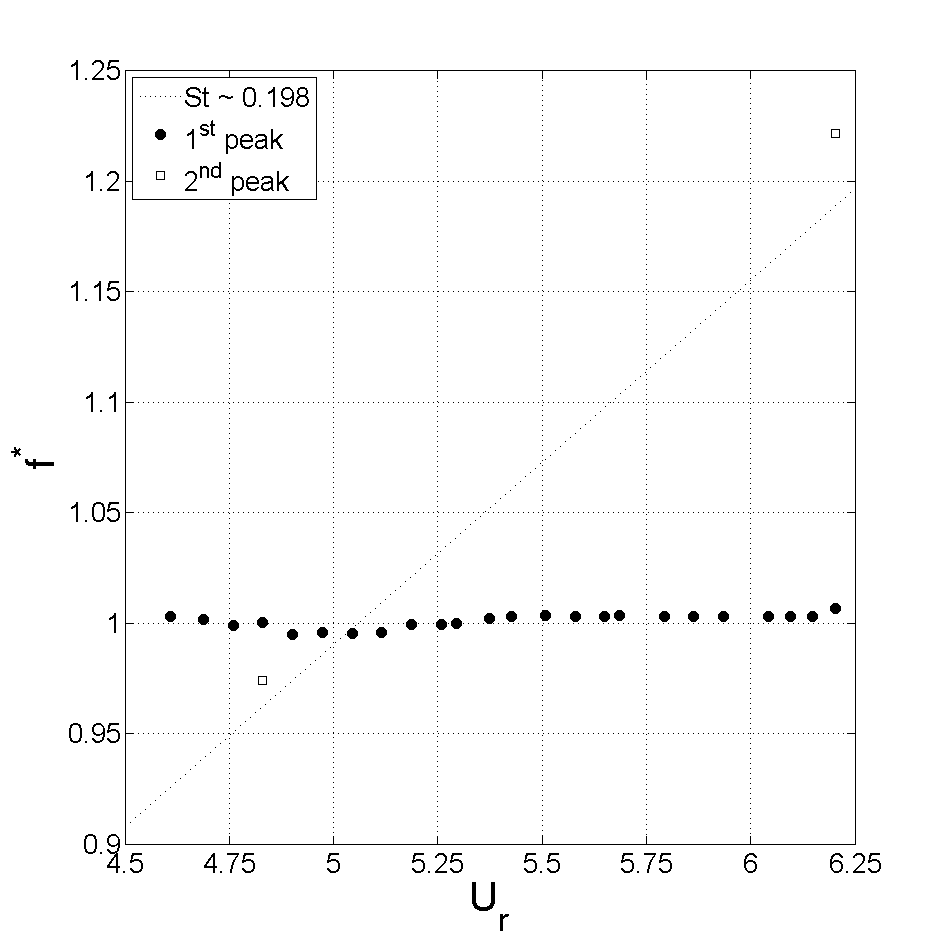
\includegraphics[width=1\textwidth]
{Figures/Fig_06_a}
{\footnotesize a)}
\end{minipage}
\begin{minipage}[r]{0.5\textwidth}
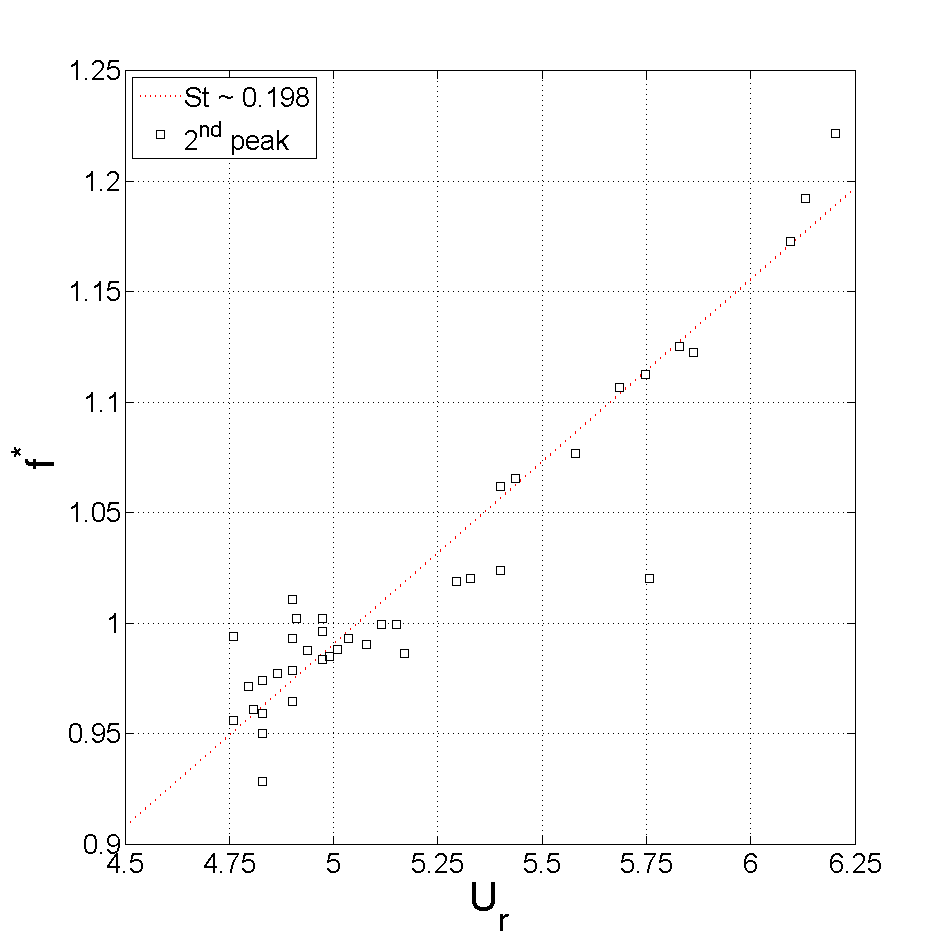
\includegraphics[width=1\textwidth]{Figures/Fig_06_b}
{\footnotesize b)}
\end{minipage}
%%%%%%%%%%%%%%%%%%%%%%
\caption{$f^*$ v.s $U_{r}$. 
a) Black circles: most energetic peaks in the spectra; white squares: second peaks; b) straight line: line that adjusts better to the observed second peaks in all the {\it Plasma-off} cases.}
\label{fig:06}
\end{minipage}
\end{center}
\end{figure}

\subsection*{PIV measurements}

PIV measurements were made for the flow in the range of reduced velocities  $U_r\in[5.2,5.5]$, considering the {\it Plasma-on} and {\it Plasma-off} cases. Each test was undertaken with an acquisition of 510 successive snapshots, suitable to achieve statistical convergence. The average time and the fluctuation intensity of the  velocity fields $\mathbf{u}(\mathbf{x})=(u_x(x,y),u_y(x,y))$ were determined respectively as:

\begin{eqnarray}
\langle\mathbf{u}(\mathbf{x})\rangle &= &\frac{1}{N}\sum_{i=1}^N \mathbf{u}(\mathbf{x},t_i) \\
\langle {u_i^{\prime}u_j^\prime}(\mathbf x)\rangle^{1/2} &=& \left[\frac{1}{N}\sum_{i=1}^N
\left(u_i(\mathbf{x},t_i)-\langle {u_i}\rangle\right)\left(u_j(\mathbf{x},t_i)-\langle {u_j}\rangle\right)\right]^{1/2}
\label{fluct_eq}
\end{eqnarray}

Figure \ref{fig:07} shows the time average velocity fields, for the controlled and uncontrolled cases, for $U_{r} = 5.2$ and  $U_{r} = 5.5$ respectively represented by streamlines and velocity contours. We find it important to recall that at the considered  Reynolds numbers, the BvK vortex street remains as the dominating flow coherent structure. In the near wake, where the flow is decelerated after the detachment, a mean recirculation region that encloses  two counter-rotating vortices can be defined. It is possible to characterise this  region with the recirculation length $\ell_m$,the distance between the cylinder and the furthest downstream point where the streamwise velocity $u_x=0$. For the unforced flow, Fig. \ref{fig:07}a, b), the values $\ell_m \approx 1.71 $ and $1.86$ are found for $U_{r}=5.2$ and $5.5$ respectively. Nevertheless, under plasma control (Fig.\ref{fig:07}c, d)), the recirculation region shortens in both cases to $\ell_m \approx 1.63$ and $1.71$. 

\begin{figure}[h]
	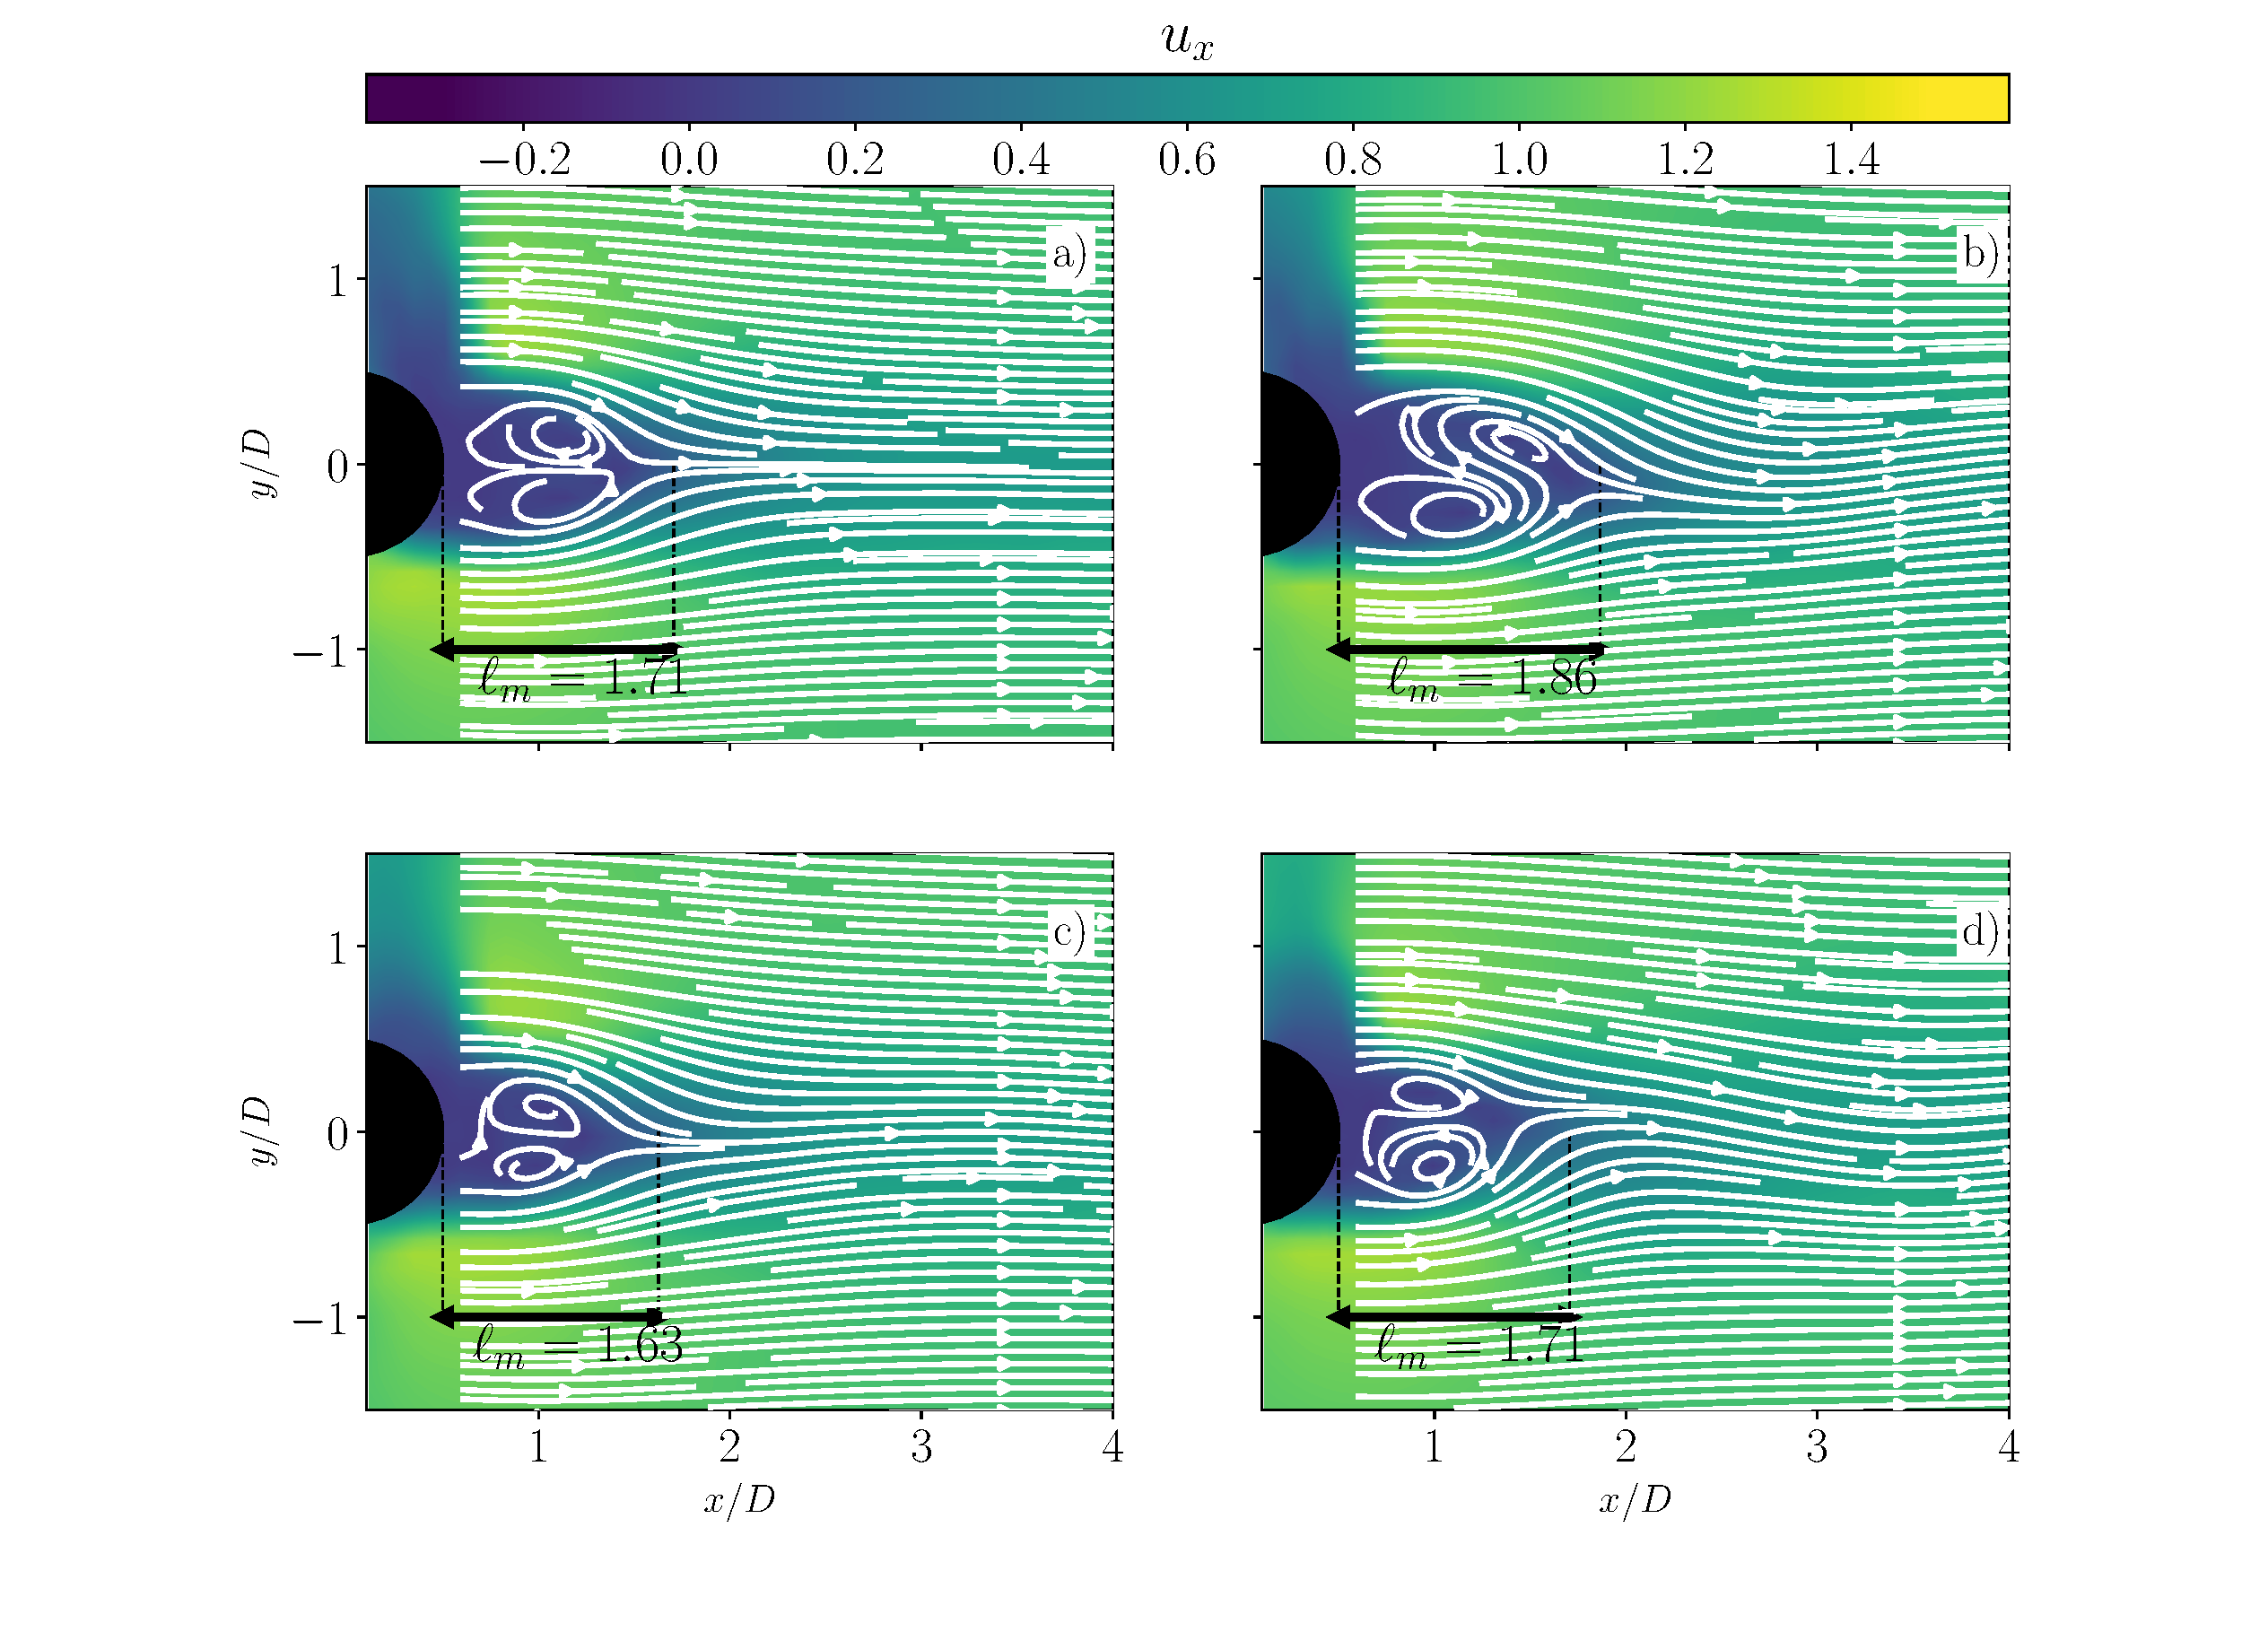
\includegraphics[width=\textwidth,trim=5mm 5mm 5mm 0mm,clip]{Figures/Fig_07}
	\caption{Streamlines and streamwise velocity $u_x$  contours in $m/s$ for a) $U_r=5.2$ plasma off; b) $U_r=5.5$ plasma off; c) $U_r=5.2$ plasma on; d) $U_r=5.5$ plasma on.}
    \label{fig:07}
\end{figure}

Figure \ref{fig:08} shows the averaged time and the fluctuations regarding intensity of the velocity profiles for the controlled and uncontrolled case when $U_r=5.5$ (similar results were found for $U_r=5.2$). The profiles are taken at positions $x/D\in[1.00,1.25,1.50,1.75]$. Consistent with the shortening of the recirculation region by plasma actuation, a narrowing of the wake and accelerations of the upstream shear layer region can be observed in the averaged time velocity profiles $\langle u_x\rangle$ in Fig. \ref{fig:08} a). Besides, further downstream, plasma actuation produces a  lower momentum deficit rather than unforced flows. The modification of recirculation region is also accompanied by an increase of the Reynolds normal and shear stresses (Fig. \ref{fig:08}b, c, d)), which corresponds to larger forces acting on a fictive control area enclosing the mean recirculation region.

\begin{figure}[h]
\centering
	\begin{overpic}[width=0.9\textwidth,trim=7mm 0mm 5mm 0mm,clip]{Figures/Fig_08}	
		\begin{small}
	\put(28,44){a)}	\put(75,44){b)}
	\put(28,0){c)}	\put(75,0){d)}		
\end{small}
\end{overpic}
	\caption{Time-averaged velocity moments profiles in $U_r=5.5$. a): $\langle {u_x}\rangle$; b): transversal $\std{u'_y}$; c): streamwise $\std{u'_x}$; d): shear Reynolds stresses $\langle u'_x u'_y\rangle^{1/2}$. The profiles are taken at positions $x/D\in[1.00,1.25,1.50,1.75]$.}
\label{fig:08}
\end{figure}

\subsubsection*{Clustering technique}

As the PIV system is not time resolved for the flow under consideration, to have relevant data of the dynamics of the flow, an indirect method was considered. For forced flows, if a regular periodicity of the flow can be well established, when lock in regimes are attained for example, it is possible to synchronise the PIV acquisition with the actuator frequency in order to perform a phase average. However, in any other condition, it is not possible to predict the characteristic frequency of the flow and therefore it is not possible to perform a phase average acquisition. Thus, instead of relying on  phase averaging techniques, a clustering technique, named \textit{k-means} algorithm, was used to classify the acquired PIV fields and obtain a number of different representative states. A brief description of the applied algorithm  can be found in \cite{dadamo2017}, further details and extensions of this method  are presented in \cite{kaiser2014}.

\begin{figure}[h]
\centering 
	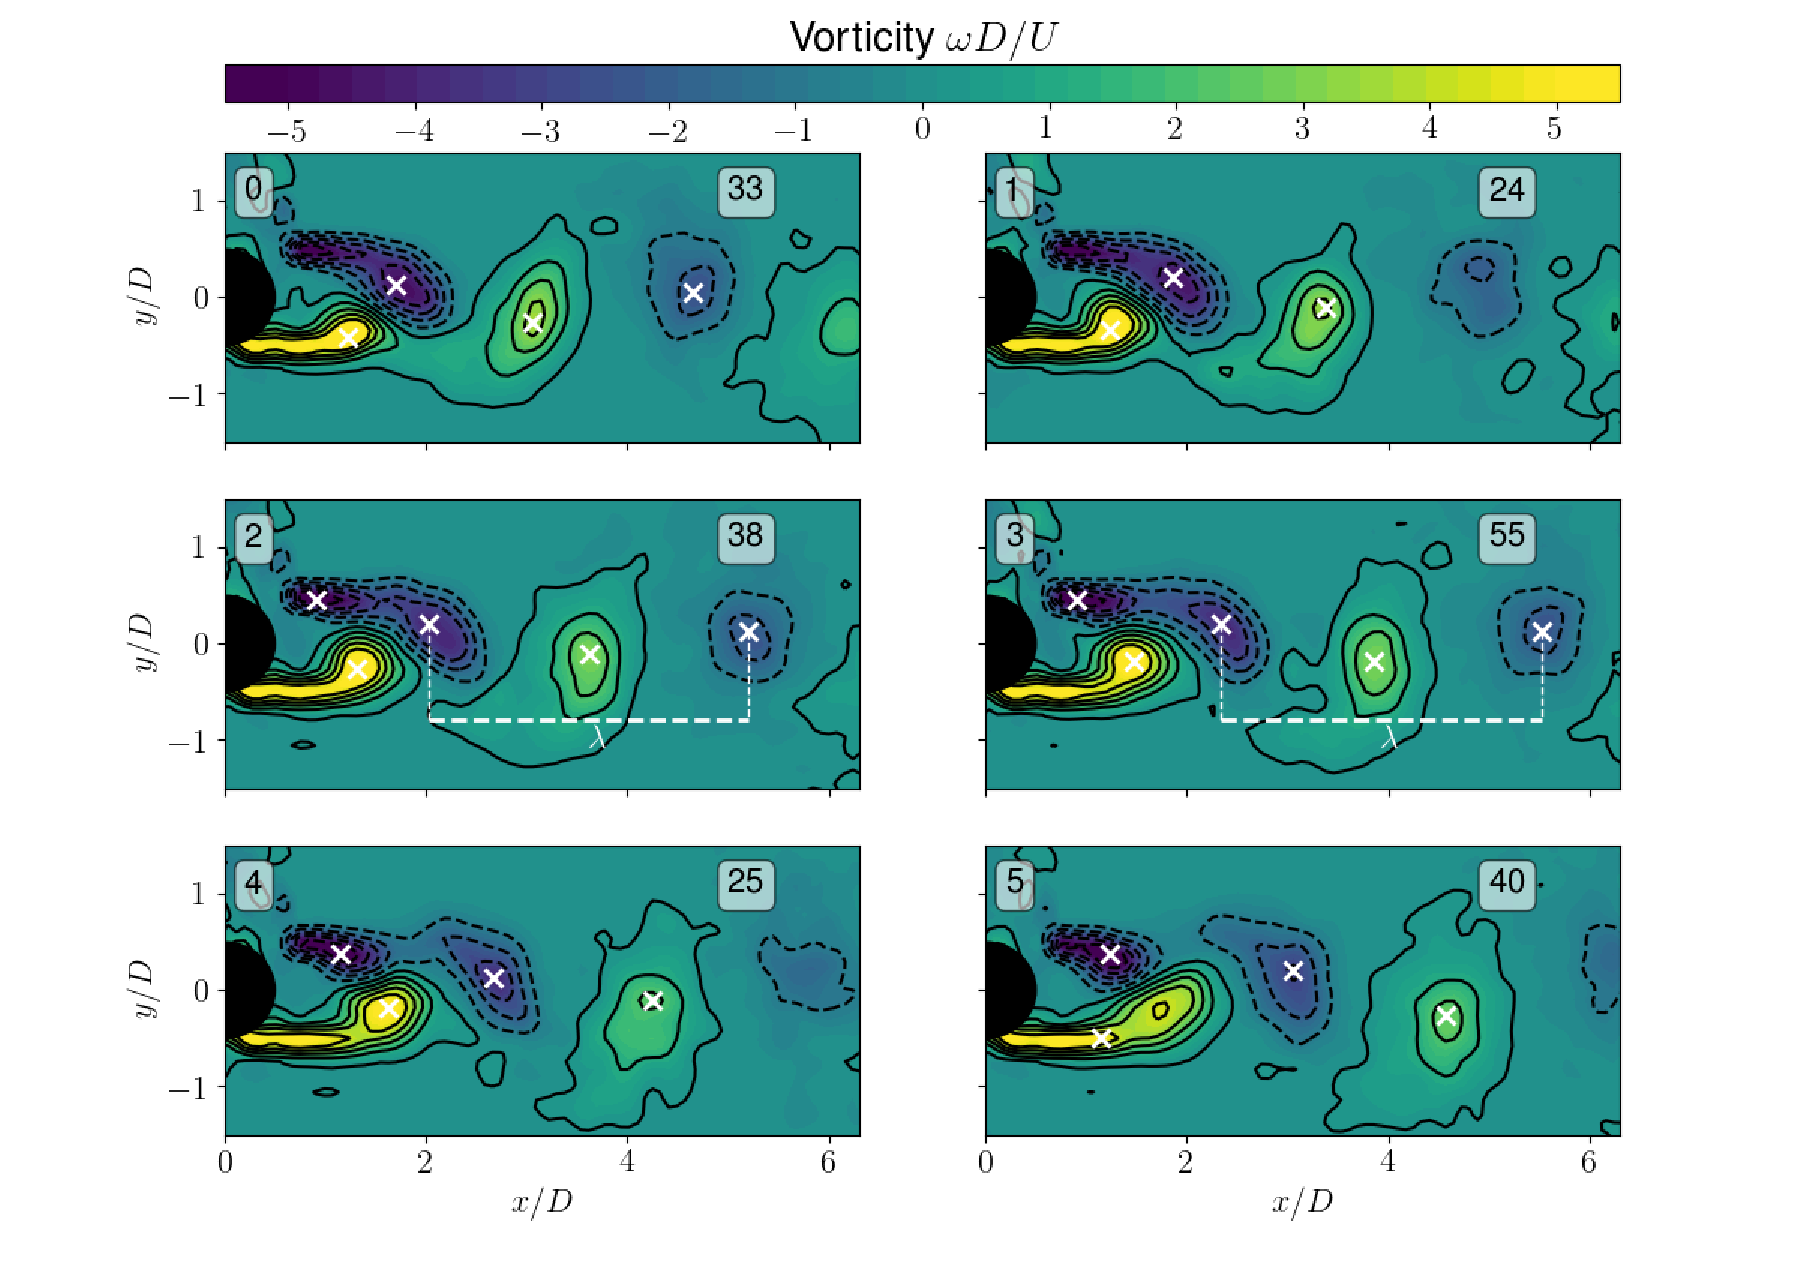
\includegraphics[width=\textwidth]{Figures/Fig_09}
	\caption{Dimensionless vorticity $\omega D/U$ contours of the clusters for $U_r=5.5$, uncontrolled case. The sequence, labeled  0 to 5 at upper left, corresponds to half a period of vortex shedding. The number of snapshots that belongs to each cluster is shown at upper right.  Vortex cores are identified with a ``$\times$" symbol. An estimation of the BvK instability wavelength $\lambda$ is showed.}
	\label{fig:09}
\end{figure}

\begin{figure}[h]
\centering 
	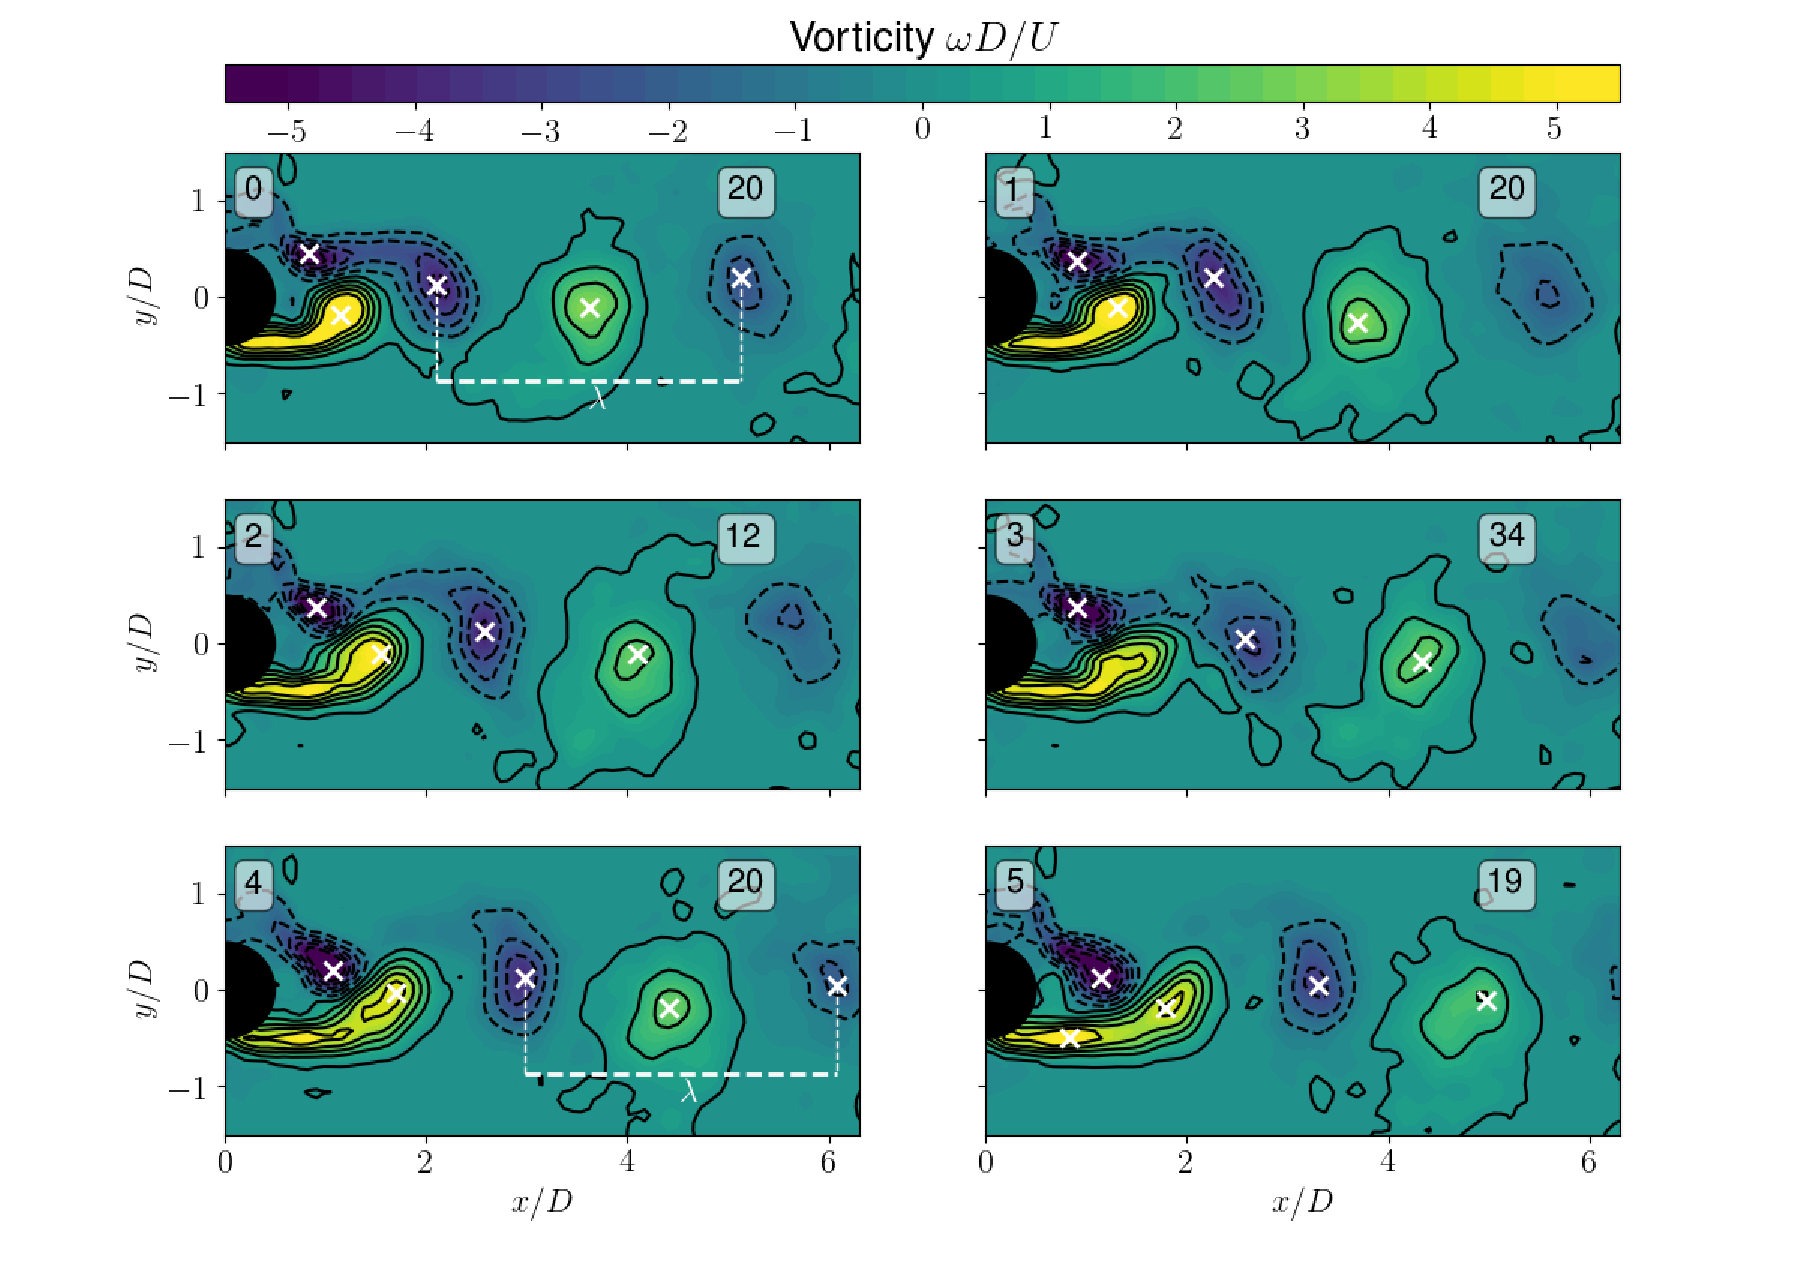
\includegraphics[width=\textwidth]{Figures/Fig_10}
	\caption{Dimensionless vorticity $\omega D/U$ contours of the cluster sequences of half a period in the controlled case for $U_r=5.5$}
	\label{fig:10}
\end{figure}

In this investigation, each cluster or representative state of the flow was constructed from, at least, 12 snapshots. We consider, in this sense, a total of $N_c=12$ clusters in order to have an insight on the flow dynamics of each studied case. Figure \ref{fig:09} shows  vorticity contours for 6 clusters (numbered 0 to 5), that represent half of the vortex shedding period dynamics that corresponds to $U_r=5.5$ without plasma control. By applying this method, the coherent structures, given by the BvK vortex street, become noticeable. The result, similar to phase averaging allow us to clearly identify vortex cores. The clusters are ordered through cross-correlation so shedding develops accordingly.

Vortex identification for planar flows can be achieved by means of positive $Q$ where  $Q=(\partial u_i / \partial x_j)( \partial u_j/\partial x_i)/2$ is the second invariant of $\nabla \mathbf u$. By detecting local minima, we have marked the cores and a wavelength $\lambda$ can be estimated. For $U_r=5.5$, $\lambda\simeq 3.3$ without flow control. In the same sense, Fig. \ref{fig:10} shows the clusters for $U_r=5.5$ with plasma control. It is clearly observed that BvK vortex street remains as the coherent structure. The wavelength is slightly smaller, as $\lambda\simeq 3.0$. 

Results shown in previous articles show that the electrohydrodynamic forcing with electrodes placed in a similar way produce a reduction of the main base pressure \citep{Artana2003}. This result was in agreement with observations of other authors that signal that forcing with this plasma actuator in a similar configuration promotes the bidimensionality of the flow \citep{Munska2005}. This leads to vortex of higher intensity and, in consequence, to an increase on the forces produced by the flow on the structure. Accordingly, we can not associate the suppression of vibrations of the cylinder to a reduction of the intensity of the forcing (vortex-strength-reduction mechanism). The only possible mechanism can be a shifting of the vortex shedding frequency away from the natural frequency of the structure. The flow can not be driven in this case by the very high frequency of the plasma and the only possible mechanism to modify the shedding frequency is an alteration of the flow instabilities phenomena associated to the vortices formation. In order to analyse possible changes in the frequency of vortex shedding as a consequence of actuation, we rely on the PIV measurements. The time averaged flow fields show significant modifications when control is on. A linear instability analysis could be proposed here to analyse how the vortex shedding frequencies could be modified. However, it becomes much more direct to determine it from experiments. Given that wave velocity $c=\lambda f$ can be retrieved from clusters velocity fields, a direct measure of vortex frequency can be obtained. So, when no control is applied, the Strouhal number is $\text {St}=0.19\pm 0.1$ while when plasma forces the wake, the number is $\text{St}=0.25\pm 0.1$ .

These results are consistent with the observed increase in frequency and subsequent shortening of the recirculation length observed for the flow regime analysed when increasing the free stream velocity. Thus, the mechanism of frequency shift promoted by alterations of the base flow (mean flow) is compatible with the results we have obtained and enables us to explain the suppression of VIV that produces the plasma actuation.

%%%%%%%%%%%%%%%%%
\section{Conclusions}
\label{sec:Conc}
%%%%%%%%%%%%%%%%%

The plasma forcing of the vibrating cylinder leads to a shorter vortex formation region compared with the case without control. The modification of recirculation region is accompanied by an increase of the Reynolds normal and shear stresses, which corresponds to larger forces acting on a fictive control area enclosing the mean recirculation region. The altered topology of the vortex formation region is accompanied by a significant change of the vortex shedding frequency which results in a total suppression of the VIV.

The intensities of the vortices that force the structure was not decreased by the actuation. The modification produced by the actuation occurs mainly in the frequency of the forcing produced by the vortices. This is a consequence of the modifications of the process of development of instabilities of the flow that is determined by the alterations produced in the base mean flow.

The ``high'' frequency of the plasma actuation was not significantly  observed in the ``slow'' dynamic behaviour of the system we studied. However, the frequency of this actuation may couple at larger Reynolds number with the vortex shedding frequency or with the one of the transition eddies. Operation of plasma actuators in the ``burst mode'' could also enable to introduce coupling  at  lower frequencies.  Future studies should focus on achieving the possibility to drive the flow with the frequency of the actuators and analyse the possibility to increase or suppress VIV in these circumstances. 

%%%%%%%%%%%%%%%%%
\section*{References}

%% References with BibTeX database:

\bibliographystyle{ieeetr}
\bibliography{mybibfile_280219}


\end{document}
